% PLANO DE TRABALHO-------------------------------------------------------------------

\chapter{PLANO DE TRABALHO}
\label{chap:planoDeTrabalho}

Este capítulo apresenta a o cronograma e a organização das atividades a serem realizadas para que o desenvolvimento do projeto, descrevendo a sequência, datas de início, fim e o objetivo a ser alcançado com a realização dela.

\section{CRONOGRAMA}

\begin{figure}[!htb]
    \centering
    \caption{Cronograma das atividades a serem realizadas no desenvolvimento do projeto}
    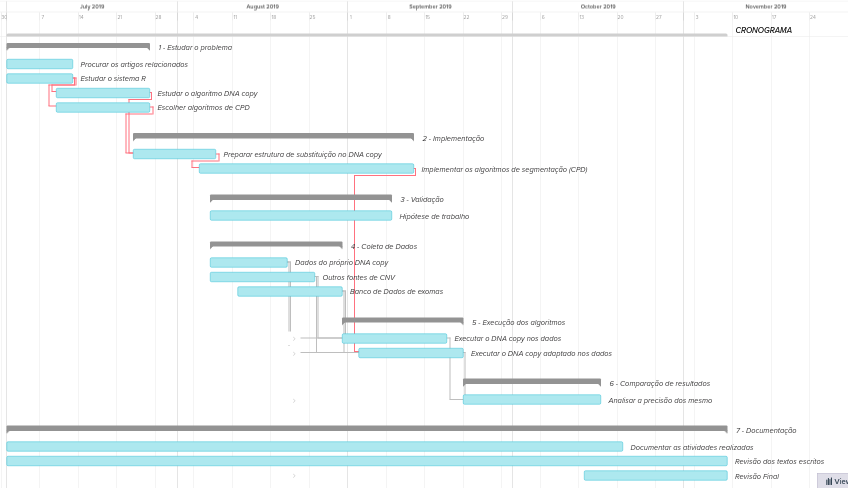
\includegraphics[width=1\textwidth]{./dados/figuras/cronograma}
    \fonte{Autoria Própria}
    \label{fig:cronograma}
\end{figure}

\subsection{Atividades do Cronograma}

O cronograma para o desenvolvimento do projeto apresenta um conjunto de sete grupos de atividades (\textit{milestones}) que representam o marco de histórico de cada uma das sub atividades que se encontram agrupadas nessa \textit{milestone}, como visto na \autoref{fig:cronograma}. A definição e levantamento desses grupos de atividades se deu ao analisar a necessidade dos requisitos e objetivos a serem atendidos para o desenvolvimento do projeto.

A seguir encontra-se uma descrição do maior grupo de atividades a serem executadas neste projeto:

\begin{enumerate}
   \item Estudar o problema
   \begin{description}
        \item[Início] 01/07/19
        \item[Fim] 26/07/19
        \item[Descrição] Investigação do assunto referente ao problema, buscando o entendimento de \textit{Change Point} e a aplicação de algoritmos de segmentação (CPD), \textit{Copy Number Variation}, linguagem R e a estrutura do DNAcopy.
    \end{description}
   \item Implementação
   \begin{description}
        \item[Início] 24/07/19
        \item[Fim] 12/09/19
        \item[Descrição] Desenvolvimento da estrutura para criação do projeto proposto, efetivando o objetivo proposto no trabalho, com a implementação da ferramenta para análise de CNV com vários algoritmos de CPD.
    \end{description}
   \item Validação
   \begin{description}
        \item[Início] 07/08/19
        \item[Fim] 08/09/19
        \item[Descrição] Definição da hipótese de trabalho e formulação da estrutura de modo a trabalhar com ela na atividade de comparação dos resultados, buscando definir a validação das funcionalidades do projeto, de acordo com a sua efetividade e desempenho.
    \end{description}
   \item Coleta de Dados
   \begin{description}
        \item[Início] 07/08/19
        \item[Fim] 30/08/19
        \item[Descrição] Busca por dados a serem utilizados como teste no projeto criado e em trabalhos de comparação com mesmo.
    \end{description}
   \item Execução dos algoritmos
   \begin{description}
        \item[Início] 31/08/19
        \item[Fim] 21/09/19
        \item[Descrição] Execução e coleta de dados gerados a partir dos testes realizados em trabalhos similares.
    \end{description}
   \item Comparação dos resultados
   \begin{description}
        \item[Início] 22/09/19
        \item[Fim] 16/10/19
        \item[Descrição] Análise dos dados da aplicação dos algoritmos testados de acordo com a Matriz de Confusão descrita na \autoref{sec:matrizDeConfusao}.
    \end{description}
   \item Documentação
   \begin{description}
        \item[Início] 01/07/19
        \item[Fim] 08/11/19
        \item[Descrição] Levantamento da escrita sobre as atividades realizadas e dados obtidos com o desenvolvimento do projeto.
    \end{description}
 \end{enumerate}